\chapter{Lec 19-20 - Minimum cut}

\section{Classification of randomized algorithms}
\begin{enumerate}
    \item Randomized algorithms that never fail. They are called \textit{LAS VEGAS} algorithms (e.g. randomized quicksort).
    \[\forall i \in I, \, A_R(i) = s \,\, \text{s.t. } (i,s) \in \Pi\]
    where $\Pi \subseteq I \times S$ is a computational problem.\newline\newline
    Randomness comes into play in the analysis of the complexity. $\forall n, \,\,T(n)$\footnote{$T(n)$ is called complexity function} is a \textbf{random variable} of which we usually study its expectation $E[T(n)]$.\newline\newline
    If $P(T(n) > c \dot f(n)) \leq \frac{1}{n^k}$ for some constants $c$ and $k$, then we say that $T(n) = O(f(n))$ \textbf{with high probability}.

    \item Randomized algorithms that may fail. They are called \textit{MONTE CARLO} algorithms (e.g. verifying polynomial identity).
    \[\forall i \in I, \,\, \text{it's possible that } A_R(i) = s \,\, \text{s.t. } (i,s) \notin \Pi\]
    We study the probability $P((i,s) \notin \Pi)$ as a function of the input size $|i| = n$.\newline\newline
    For decision problems, these algorithms can be divided in two classes:
    \begin{itemize}
        \item \textbf{One-sided:} They may fail only on one answer.

        \item \textbf{Two-sided:} They may fail in both answer.
    \end{itemize}
\end{enumerate}

\section{Terminology}
\textbf{Definition:} Given a computational problem $\Pi \subseteq I \times S$, an algorithm $A_\Pi$ has complexity $T(n) = O(f(n))$ \textbf{with high probability} (w.h.p.) if $\exists$ constants $c, d > 0$ such that $\forall i \in I$ of size $n$ the following probability holds:
\[P(A_\Pi(i)\,\, \text{terminates in $> c\cdot f(n)$ steps}) \leq \frac{1}{n^d}\]
Then the probability of having a complexity of $O(f(n))$ is $> 1 - \frac{1}{n^d}$, that is, tends to 1 as $n$ tends to $\infty$.\newline\newline
\textbf{Definition:} Given a computational problem $\Pi \subseteq I \times S$, an algorithm $A_\Pi$ is correct w.h.p. if $\exists$ constant $d > 0$ such that $\forall i \in I, \,\, |i| = n$:
\[P((i, A_\Pi(i)) \notin \Pi) \leq \frac{1}{n^d}\]
\textbf{Markov's lemma:} Let $T$ be a non-negative, bounded ($\exists b \in \mathbb{N} \,\, \text{s.t. } P(T > b) = 0$), integer random variable. Then, $\forall t \,\, \text{such that } 0 \leq t \leq b$:
\[t \cdot P(T \geq t) \leq E[T] \leq t + (b - t)P(T \geq t)\]
\textbf{Application of Markov's lemma:}
Given a \textit{LAS VEGAS} algorithm $A_\Pi$, assume that:
\begin{enumerate}
    \item $T_{A_\Pi}(n) = O(f(n))$ with high probability, in particular, $P(T_{A_\Pi}(n) > c \cdot f(n)) \leq \frac{1}{n^d}$.

    \item $A_\Pi$ has a worst-case deterministic complexity $O(n^a), \,\, a \leq d \,\, \forall n$
\end{enumerate}
We can use Markov's lemma to prove the following property:
\[E[T_{A_\Pi}(n)] = O(f(n))\]
\textbf{Proof:} Just apply Markov's lemma:
\[E[T_{A_\Pi}(n)] \leq c \cdot f(n) + (n^a - c \cdot f(n)) \cdot \frac{1}{n^d} \leq c \cdot f(n) + \frac{n^a}{n^d} \leq c \cdot f(n) + 1\]
where:
\begin{itemize}
    \item $c \cdot f(n)$ is $t$
    \item $(n^a - c \cdot f(n))$ is $b - t$
    \item $\frac{1}{n^d}$ is $P(T \geq t)$
\end{itemize}


\section{Karger's algorithm for Minimum cut}
The minimum cut problem is finding a cut of minimum size, that is, the minimum number of edges whose removal disconnects the graph.\newline\newline
Karger's algorithm actually solves a more general problem: minimum cut on \textbf{multigraphs} (i.e. multiple edges between two vertices are allowed).\newline\newline
\textbf{Definition:} A \textbf{multiset} is a collection of objects with repetitions allowed.
\[S = \{\{\text{objects}\}\}\]
where $\forall \, \text{object }o \in S$, $m(o) \in \mathbb{N} \setminus \{0\}$ is called multiplicity, that is, how many copies of $o$ are in $S$.\newline\newline
\textbf{Definition:} We denote a multigraph as follows: $G = (V, E)$ where $V \subseteq \mathbb{N}$ and $E$ is a multiset of elements $(u,v)\,\, u \neq v$.\newline\newline
\textbf{Example:}\newline\newline
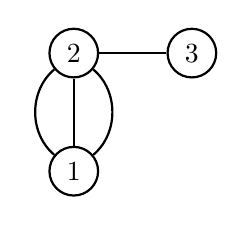
\begin{tikzpicture}[node distance={15mm}, thick, main/.style = {draw, circle}] 
            \node[main] (1) {$1$}; 
            \node[main] (2) [above of=1] {$2$}; 
            \node[main] (3) [right of=2] {$3$}; 

            \draw (1) edge[bend right = 50] (2); 
            \draw (1) -- (2); 
            \draw (1) edge[bend left = 50] (2);
            \draw (2) -- (3);
\end{tikzpicture}\newline\newline
A simple graph is also a multigraph.\newline\newline
\textbf{Definition:}Given a connected multigraph $G = (V, E)$. A cut $C \subseteq E$ is a multiset of edges such that $G' = (V, E \setminus C)$ is not connected.\newline\newline
\textbf{Karger's algorithm (simplified version):}
\begin{enumerate}
    \item Choose an edge at random;
    \item \textit{Contract} the two vertices of that edge;
    \item Repeat until only two vertices remain;
    \item Return the edges between them;
\end{enumerate}
\textbf{Definition:} Given a multigraph $G=(V,E)$ and an edge $e = (u, v)$, the \textbf{contraction} of $G$ with respect to $e$ is: $G_{/e} = (V', E')$ where:
\begin{itemize}
    \item $V' = V \setminus \{u, v\} \cup \{z_{u,v}\}$ where $z_{u,v} \notin V$.

    \item $E' = E \setminus \{\{ (x,y) : (x = u)\,\, \text{or}\,\, (x = v)\}\} \cup \{\{ (z_{u,v}, y) : (u, y) \in E \,\, \text{or} \,\, (v, y) \in E, \,\, y \neq u \,\, \text{and} \,\, y \neq v   \}\}$
\end{itemize}
It follows that:
\begin{itemize}
    \item $|V'| = |V| - 1$

    \item $|E'| = |E| - m(e) \leq |E| - 1$
\end{itemize}
Basically, it makes the two vertices to collapse in just one vertex connected with all the previous adjacent vertices. If as a result there are several edges between some pairs of (newly formed) vertices, retain them all.\newline\newline
\textbf{Example:}\newline\newline
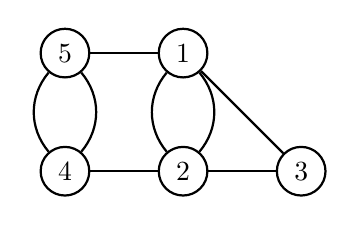
\begin{tikzpicture}[node distance={15mm}, thick, main/.style = {draw, circle}] 
            \node[main] (1) {$1$}; 
            \node[main] (2) [below of=1] {$2$}; 
            \node[main] (3) [right of=2] {$3$};
            \node[main] (4) [left of=2] {$4$};
            \node[main] (5) [above of=4] {$5$}; 

            \draw (1) edge[bend right = 40] (2); 
            \draw (1) edge[bend left = 40] (2);
            \draw (2) -- (3);
            \draw (1) -- (3);
            \draw (5) -- (1);
            \draw (4) -- (2);
            \draw (4) edge[bend right = 40] (5); 
            \draw (4) edge[bend left = 40] (5);
\end{tikzpicture}\newline\newline
The contraction of $G$ with respect to the edge $(1,2)$ is the following:\newline\newline
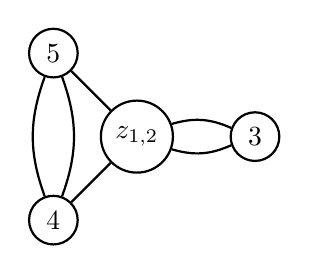
\begin{tikzpicture}[node distance={15mm}, thick, main/.style = {draw, circle}] 
            \node[main] (z) {$z_{1,2}$};
            \node[main] (3) [right of=z] {$3$};
            \node[main] (4) [below left of=z] {$4$};
            \node[main] (5) [above left of=z] {$5$}; 


            \draw (z) edge[bend right = 20] (3);
            \draw (z) edge[bend left = 20] (3);
            \draw (5) -- (z);
            \draw (4) -- (z);
            \draw (4) edge[bend right = 20] (5); 
            \draw (4) edge[bend left = 20] (5);
\end{tikzpicture}\newline\newline
Actually, the probability that at the first run Karger's algorithm returns a minimum cut is \textbf{not} high. The idea is to repeat the procedure $k$ times to reduce the probability of error. The value of $k$ will be determined by the analysis of the algorithm.\newpage
\begin{algorithm}
\caption{Karger's algorithm}\label{KARGER}
    \begin{algorithmic}[1]
    \Procedure{Karger($G, k$)}{}
        \State $min = \infty$
        \For{$i = 1$ to $k$}
            \State $t =$ \textit{FULL\_CONTRACTION($G$)}
            \If{$t < min$}
                \State $min = t$
            \EndIf
        \EndFor
        \Return $min$
    \EndProcedure   
    \end{algorithmic}
\end{algorithm}

\begin{algorithm}
\caption{FULL\_CONTRACTION}\label{FULLC}
    \begin{algorithmic}[1]
    \Procedure{FULL\_CONTRACTION($G = (V, E)$)}{}
        \For{$i = 1$ to $n - 2$}
            \State $e = $ random($E$)
            \State $G' = (V', E') = G_{/e} \quad \text{//Contraction}$
            \State $V = V'$
            \State $E = E'$
        \EndFor
        \Return $|E|$
    \EndProcedure   
    \end{algorithmic}
\end{algorithm}
\section{Analysis of Karger's algorithm}
We'll show for which value of $k$ the algorithm returns a minimum cut with high probability.\newline\newline
\textbf{Property:} $\forall$ cut $C'$ in $G_{/e}$ $\exists$ a cut $C$ in $G$ of the same cardinality.\newline\newline
This implies that $|\text{minimum cut in }G_{/e}| \geq |\text{minimum cut in } G|$.\newline\newline
\textbf{Proof:}Given a cut $C'$ in $G_{/e}$, the idea is to determine the corresponding cut $C$ in $G$ by substituting each edge $(z_{u, v}, y)$ in $C'$ with $(u, y)$ or $(v, y)$. Then, it remains to show that $C$ is a cut in $G$.\newline\newline
Let $C'$ be a cut in $G_{/e} = (V', E')$. Then, $C'$ separates $V'$ in 2 connected components. Let $V_1 \subset V'$ the connected component containing $z_{u,v}$, and let $x \notin V_1$. Then, in $G_{/e}$ every path from $z_{u, v}$ to $x$ must use an edge in $C'$.\newline\newline
Now we'll show that $C$ in $G$ disconnects $u$ and $v$ from $x$. Assume by contradiction that $C$ is \textbf{not} a cut in $G$. This implies that it exists a path between $u$ and $x$ after the removal of $C$ from $E$. Then, the path between $z_{u, v}$ and $x$ \textit{survives} the removal of $C'$ in $G_{/e}$. This implies that $C'$ is not a cut in $G_{/e} \rightarrow$ contradiction!\newline\newline
Note that the cuts that disappear in the contracted graph are the ones hit by the random choice of the edge $e$, all the others are preserved. This means that the only time the algorithm fails is when an edge belonging to a minimum cut in $G$ is hit by the random choice. Basically, by proving the property above we have shown that, if the algorithm never hits an edge belonging to a minimum cut, then it returns a correct solution (because the minimum cut is preserved in $G_{/e}$).\newline\newline
Therefore, we want the probability of \textbf{not} hitting edges of the minimum cut to be sufficiently high.

\subsection{Conditional probability recall}
\textbf{Definition:} The events $E_1, E_2$ are \textbf{independent} if:
\[P(E_1 \cap E_2) = P(E_1) \cdot P(E_2)\]
\textbf{Definition:} Given $P(E_1) > 0$, then:
\[P(E_2 | E_1) = \frac{P(E_1 \cap E_2)}{P(E_1)}\]
extension to $k$ events:
\[P(E_1 \cap E_2 \cap E_3 \cap ... \cap E_k) = P(E_1)P(E_2 | E_1)P(E_3 | E_1 \cap E_2) ... P(E_k | E_1 \cap ... \cap E_{k-1})\]

\subsection{Analysis of \textit{FULL\_CONTRACTION}}
\textbf{Intuition:} Since $|\text{min. cut}|$ is a small portion of $|E|$, it is \textit{unlikely} to hit an edge of a minimum cut. Let's calculate what is this probability.\newline\newline
\textbf{Property:} Let $G=(V, E), \,\, |V| = n$. If $G$ has a minimum cut of size $t$, then $|E| \geq t \cdot \frac{n}{2}$.\newline\newline
\textbf{Proof:} $d(v) \geq t \,\, \forall v \in V$. This is because If we take a node and remove all the edges incident to that node, that's a cut.
\[
    \begin{split}
        \sum_{v \in V}d(v) & = 2m \geq t \cdot n\\
        m & = |E| \geq \frac{t \cdot n}{2}
    \end{split}
\]
Let $t = |\text{minimum cut}|$. Given the event $E_i = \text{in the i-th contruction i did \textbf{not} hit an edge of the minimum cut}$, it follows that:
\[
    \begin{split}
        P(\overline{E}_1) & = \frac{t}{|E|} \leq \frac{t}{t \cdot \frac{n}{2}} = \frac{2}{n}\\
        P(\overline{E}_1) & \leq \frac{2}{n}\\
        P(E_1) & \geq 1 - \frac{2}{n}\\
    \end{split}
\]
Since after every contruction $|V'| = |V| - 1$, the following holds:
\[
    \begin{split}
        P(E_2 | E_1) & \geq 1 - \frac{t}{t \cdot \frac{(n - 1)}{2}} = 1 - \frac{2}{n - 1}\\
        & ... \\
        P(E_i | E_1 \cap ... \cap E_{i-1}) & \geq 1 - \frac{t}{\frac{t(n- i + 1)}{2}} = 1 - \frac{2}{n - i + 1}
    \end{split}
\]
Therefore, the probability that \textit{FULL\_CONTRUCTION} succeeds becomes:
\[
    \begin{split}
        P(\textit{FULL\_CONTRUCTION succeeds}) & \geq P(\bigcap_{i = 1}^{n-2}E_i) = \prod_{i = 1}^{n - 2}\left(1 - \frac{2}{n - i + 1}\right) = \prod_{i = 1}^{n-2} \frac{n - i -1}{n - i + 1}\\
        & \geq \frac{\cancel{n - 2}}{n} \cdot \frac{\cancel{n - 3}}{n - 1} \cdot \frac{\cancel{n - 4}}{\cancel{n - 2}} \cdot\cdot\cdot \frac{\cancel{3}}{\cancel{5}}\cdot\frac{2}{\cancel{4}}\cdot\frac{1}{\cancel{3}} = \frac{2}{n(n - 1)}
    \end{split}
\]
Basically, the probability that \textit{FULL\_CONTRUCTION} does not hit an edge of a minimum cut is at least $\frac{2}{n^2}$. Not so good as a bound. Our algorithm may err
in declaring the cut it outputs to be a min-cut. Karger's amplifies this probability by repeating \textit{FULL\_CONTRUCTION} multiple times:
\[P(\textit{the k runs of FULL\_CONTRUCTION do not return the minimum cut}) \leq \left(1 - \frac{2}{n^2}\right)^{k}\]
We want to find a value for $k$ such that $\left(1 - \frac{2}{n^2}\right)^{k} \leq \frac{1}{n^d}$. In order to do this, we'll use the following two rules:
\begin{itemize}
    \item $(1 + \frac{x}{y})^y \leq e^x \,\, y \geq 1, y \geq x$
    \item $e^{-ln\,n} = \frac{1}{n}$
\end{itemize}
By choosing $k = d\frac{n^2}{2}ln\,n$, it follows that:
\[
    \begin{split}
        & = \left(\left(1 - \frac{2}{n^2}\right)^{n^2}\right)^{\frac{d}{2}ln\, n}\\
        & \leq (e^{-2})^{\frac{d}{2}ln\, n} = e^{-ln\, n^d} = \frac{1}{n^d}
    \end{split}
\]
Then, by choosing that value for $k$ the Karger's algorithm succeeds with high probability:
\[P(\textit{Karger's succeeds}) \geq 1 - \frac{1}{n^d}\]

\subsection{Complexity}
\textit{FULL\_CONTRUCTION} can be implemented in $O(n^2)$. Then, the complexity of Karger's algorithm is $O(n^4log\, n)$. It is not very fast, but it can be improved to obtain a complexity of $O(n^2log^3\,n)$.\newline\newline
The fastest algorithm for this problem has a complexity of $O(m log\,n)$.
